\documentclass[tikz,border=5pt]{standalone}
\usepackage[T1]{fontenc}
\usepackage{lmodern,amsmath,amssymb}
\usetikzlibrary{arrows.meta,calc,positioning,fit,backgrounds,shapes.geometric,matrix,decorations.pathreplacing,patterns}
\definecolor{ink}{gray}{0.08}
\definecolor{wash}{gray}{0.965}
\definecolor{soft}{gray}{0.45}
\tikzset{box/.style={draw=ink,line width=.65pt,fill=white,align=center,inner sep=4pt,outer sep=0pt,font=\small},flow/.style={draw=ink,line width=.65pt,-{Latex[length=1.8mm,width=1.3mm]},rounded corners=2pt},annotation/.style={font=\scriptsize,text=soft,align=center},groupbox/.style={draw=soft,dashed,line width=.45pt,fill=wash}}
\begin{document}
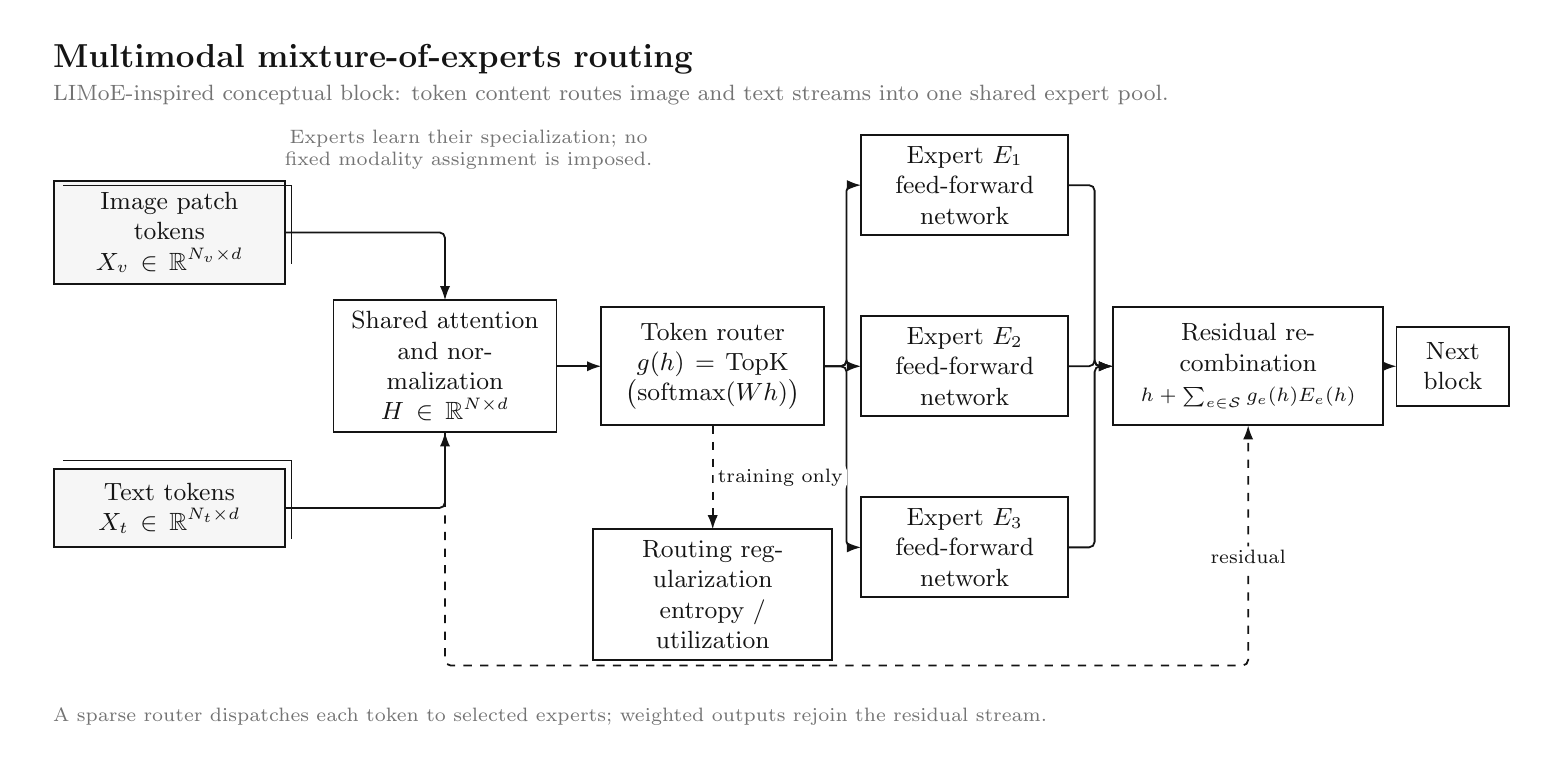
\begin{tikzpicture}[x=1cm,y=-1cm,font=\rmfamily,text=ink]

\path[use as bounding box] (0,0) rectangle (19,9);
\node[anchor=west,font=\large\bfseries] at (.2,.4) {Multimodal mixture-of-experts routing};
\node[anchor=west,font=\footnotesize,text=soft] at (.2,.85) {LIMoE-inspired conceptual block: token content routes image and text streams into one shared expert pool.};
\begin{pgfonlayer}{background}
\end{pgfonlayer}
\node[box,fill=wash,minimum width=2.9cm,minimum height=1.0cm,text width=2.65cm] (image) at (1.8,2.6) {Image patch tokens\\$X_v\in\mathbb{R}^{N_v\times d}$};
\draw[ink,line width=.4pt] (0.45000000000000007,2.0) -- (3.35,2.0) -- (3.35,3.0);
\node[box,fill=wash,minimum width=2.9cm,minimum height=1.0cm,text width=2.65cm] (text) at (1.8,6.1) {Text tokens\\$X_t\in\mathbb{R}^{N_t\times d}$};
\draw[ink,line width=.4pt] (0.45000000000000007,5.5) -- (3.35,5.5) -- (3.35,6.5);
\node[box,minimum width=2.8cm,minimum height=1.5cm,text width=2.55cm] (shared) at (5.3,4.3) {Shared attention\\and normalization\\$H\in\mathbb{R}^{N\times d}$};
\node[box,minimum width=2.8cm,minimum height=1.5cm,text width=2.55cm] (router) at (8.7,4.3) {Token router\\$g(h)=\mathrm{TopK}$\\$\bigl(\mathrm{softmax}(Wh)\bigr)$};
\node[box,minimum width=2.6cm,minimum height=1.0cm,text width=2.35cm] (expert1) at (11.9,2.0) {Expert $E_{1}$\\feed-forward network};
\node[box,minimum width=2.6cm,minimum height=1.0cm,text width=2.35cm] (expert2) at (11.9,4.3) {Expert $E_{2}$\\feed-forward network};
\node[box,minimum width=2.6cm,minimum height=1.0cm,text width=2.35cm] (expert3) at (11.9,6.6) {Expert $E_{3}$\\feed-forward network};
\node[box,minimum width=3.4cm,minimum height=1.5cm,text width=3.15cm] (combine) at (15.5,4.3) {Residual recombination\\{\scriptsize $h+\sum_{e\in\mathcal S}g_e(h)E_e(h)$}};
\node[box,minimum width=1.4cm,minimum height=1.0cm,text width=1.15cm] (out) at (18.1,4.3) {Next\\block};
\node[box,minimum width=3.0cm,minimum height=0.9cm,text width=2.75cm] (aux) at (8.7,7.2) {Routing regularization\\entropy / utilization};
\begin{pgfonlayer}{background}
\draw[flow] (router.east) -- (10.4,4.3) -- (10.4,2.0) -- (expert1.west);
\draw[flow] (router.east) -- (10.4,4.3) -- (10.4,4.3) -- (expert2.west);
\draw[flow] (router.east) -- (10.4,4.3) -- (10.4,6.6) -- (expert3.west);
\draw[flow] (image.east) -- (5.3,2.6) -- (shared.north);
\draw[flow] (text.east) -- (5.3,6.1) -- (shared.south);
\draw[flow] (shared.east) -- (router.west);
\draw[flow] (expert1.east) -- (13.55,2.0) -- (13.55,4.3) -- (combine.west);
\draw[flow] (expert2.east) -- (13.55,4.3) -- (13.55,4.3) -- (combine.west);
\draw[flow] (expert3.east) -- (13.55,6.6) -- (13.55,4.3) -- (combine.west);
\draw[flow] (combine.east) -- (out.west);
\draw[flow,dashed] (router.south) -- (aux.north) node[midway,right,fill=white,inner sep=1.5pt,font=\scriptsize] {training only};
\draw[flow,dashed] (shared.south) -- (5.3,8.1) -- (15.5,8.1) -- (combine.south) node[midway,below,fill=white,inner sep=1.5pt,font=\scriptsize] {residual};
\end{pgfonlayer}
\node[annotation,text width=8.5cm] at (5.6,1.55) {Experts learn their specialization; no fixed modality assignment is imposed.};
\node[anchor=west,align=left,font=\scriptsize,text=soft,text width=18.6cm] at (.2,8.75) {A sparse router dispatches each token to selected experts; weighted outputs rejoin the residual stream.};
\end{tikzpicture}
\end{document}
